\documentclass[11pt]{article}
\usepackage{graphicx}
\usepackage{float}
\usepackage[labelformat= empty]{caption}

\title{ System Architecture Document}
\author{ Kenan Karavoussanos \\ Shaylin Pillay \\ Preshen Goobiah \\ Marc Karp}
\date{\today}
\begin{document}
\maketitle
\tableofcontents

%\bibliographystyle{plain}
\newpage
\section{Introduction}
This introduction provides a brief overview of System Architecture Document for the current iteration of the Post Graduate Application Approval System. It consists of the purpose, scope, problem statement,project objectives, stakeholders and overview of the rest of the document.
\subsection{Purpose}
\paragraph{}This document provides the reader with an architectural overview of the Post Graduate Application Approval System. The primary purpose of this project is to create a single integrated system that facilitates application review and decision making.

\paragraph{}This document is intended to elucidate the major architectural decisions that have been made when designing and implementing the system. This is achieved by viewing the system architecture from various perspectives, called views. These views are intended to explain the system architecture through all levels of the development stack, from front-end to back-end.


\subsection{Scope}
The scope of this document is the design and implementation of the software based Post Graduate Application Approval System which consists of the application upload by the Post Graduate Officer, the intermediary application review by the Supervisor and the final application review made by the Post Graduate Coordinator.


\subsection{Overview}
The rest of the document will briefly discuss the architectural goals and constraints of the environment followed by a brief description of the chosen architectural views and patterns. The architectural views will then be displayed in detail. Finally, the performance evaluation of the system and a description of the software testing will be discussed.

\section{Architectural Goals and Constraints}
The architecture of the system has been designed to achieve the following objectives:
\begin{enumerate}
	\item To assist the application approval process by having all application documents and information in a single digital repository.
	\item To assist the Post Graduate Officer with the upload of application documents.
	\item To simplify application reviews by having a single integrated view of all important information for each decision maker.
	\item To prevent human error by providing notifications and weekly reminders about pending applications.
	
\end{enumerate}

The significant constraints kept in mind when developing the system were as follows:

\begin{enumerate}
	\item Security
\item Ease of Use
\item Paperless
\end{enumerate}
\section{Architectural Representation}
\subsection{Architectural Views}
The development of the system has various contributors each with their own priorities and tasks. As such, the system needs to be documented from various perspectives to aid, and eventually validate, the completion of a contributor's tasks. The system architecture shall be represented from the following views:

\begin{enumerate}
\item Use Case View: This defines the high-level interactions between various actors and the system.
\item Design View: This contains the class and architecture diagrams of the system.
\item Process View: This displays the processes within the system that combine to perform the various interactions defined in the Use Case View.
\item Component View: This displays the User Interface of the system.
\item Database View: This contains the Entity-Relationship Diagram for the system database.
\end{enumerate} 
\subsection{Architectural Design Patterns}
ASP.NET Core framework was used in the implementation of the system. This follows the Model-View-Controller(MVC) design pattern. This design pattern separates the project into three distinct layers:

\begin{enumerate}
	\item Model: Defines the data structures of the system and directly handles all logic and data within the system. A model class communicates exclusively with its controller.
	\item View: A visual representation of a model. Typically in the form of a web page or a component of the web page. The view communicates exclusively with its controller.
	\item Controller: Accepts user input and maps it to instructions for models, views and potentially other controllers. Directly responsible for communication between components of the system.
	
	  
\end{enumerate} 

This framework and design pattern was chosen to enhance modularity of the system. This allows for: 
\begin{itemize}
	\item Parallel development
	\item Efficient code reuse
	\item Faster bug detection and tracking.
	\item Greater unit testing coverage.
	
\end{itemize} 
 
\section{Architectural View Decomposition}
\subsection{Use-Case View}
\begin{figure}[H]
	\frame{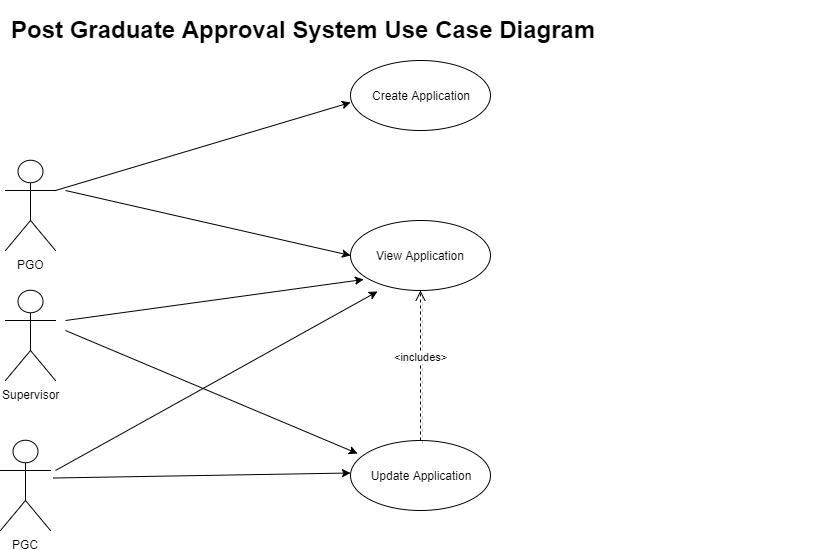
\includegraphics[width=\textwidth, height=\textheight, keepaspectratio]{Diagrams/PGASUseCases}}
	\caption{Use Case Diagram}
\end{figure}
\subsubsection{Use Case Narrative}
describe in detail the use cases that use the most critical part of the system (possibly fully dressed use cases for this)
\subsection{Design View}
\subsubsection{Class Diagram}
\begin{figure}[H]
	\frame{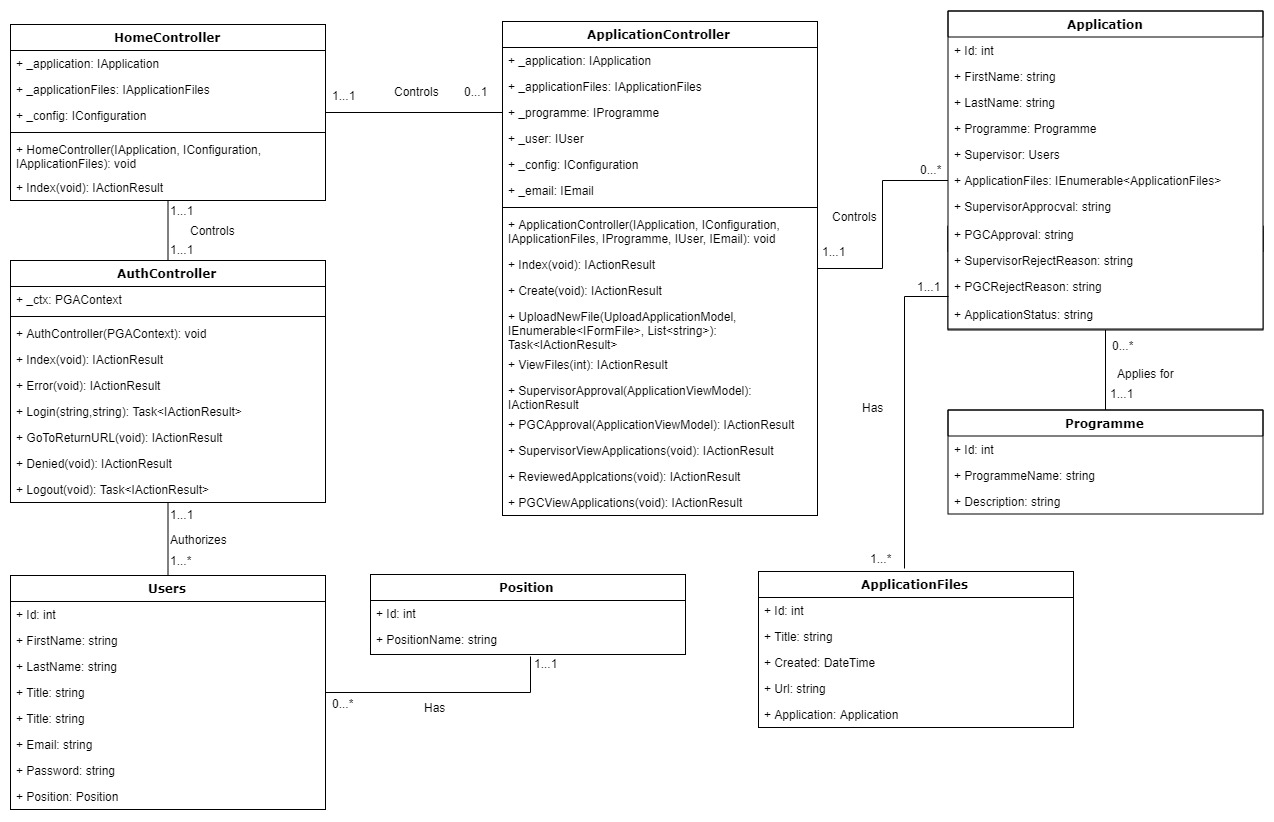
\includegraphics[width=\textwidth, height=\textheight, keepaspectratio]{Diagrams/ClassDiagram}}
	\caption{Class Diagram}
	
\paragraph{Description}
The classes are described as follows:
\begin{itemize}
	\item AuthController: Handles authentication and displays the login page.
	\item HomeController: The Controller for the home screens.
	\item ApplicationController: Handles all Application related operations i.e create, view, update.
	\item Application: The data structure that stores an application.
	\item Programme: Stores the application's course option.
	\item ApplicationFiles: Stores file metadata and the URL to the file on the Blob storage server.
	\item Users: Stores system user data.
	\item Position: Stores a user's position i.e PGO, Supervisor or PGC.
\end{itemize}
\end{figure}
\subsubsection{Hardware Architecture Diagram}
\begin{figure}[H]
	\frame{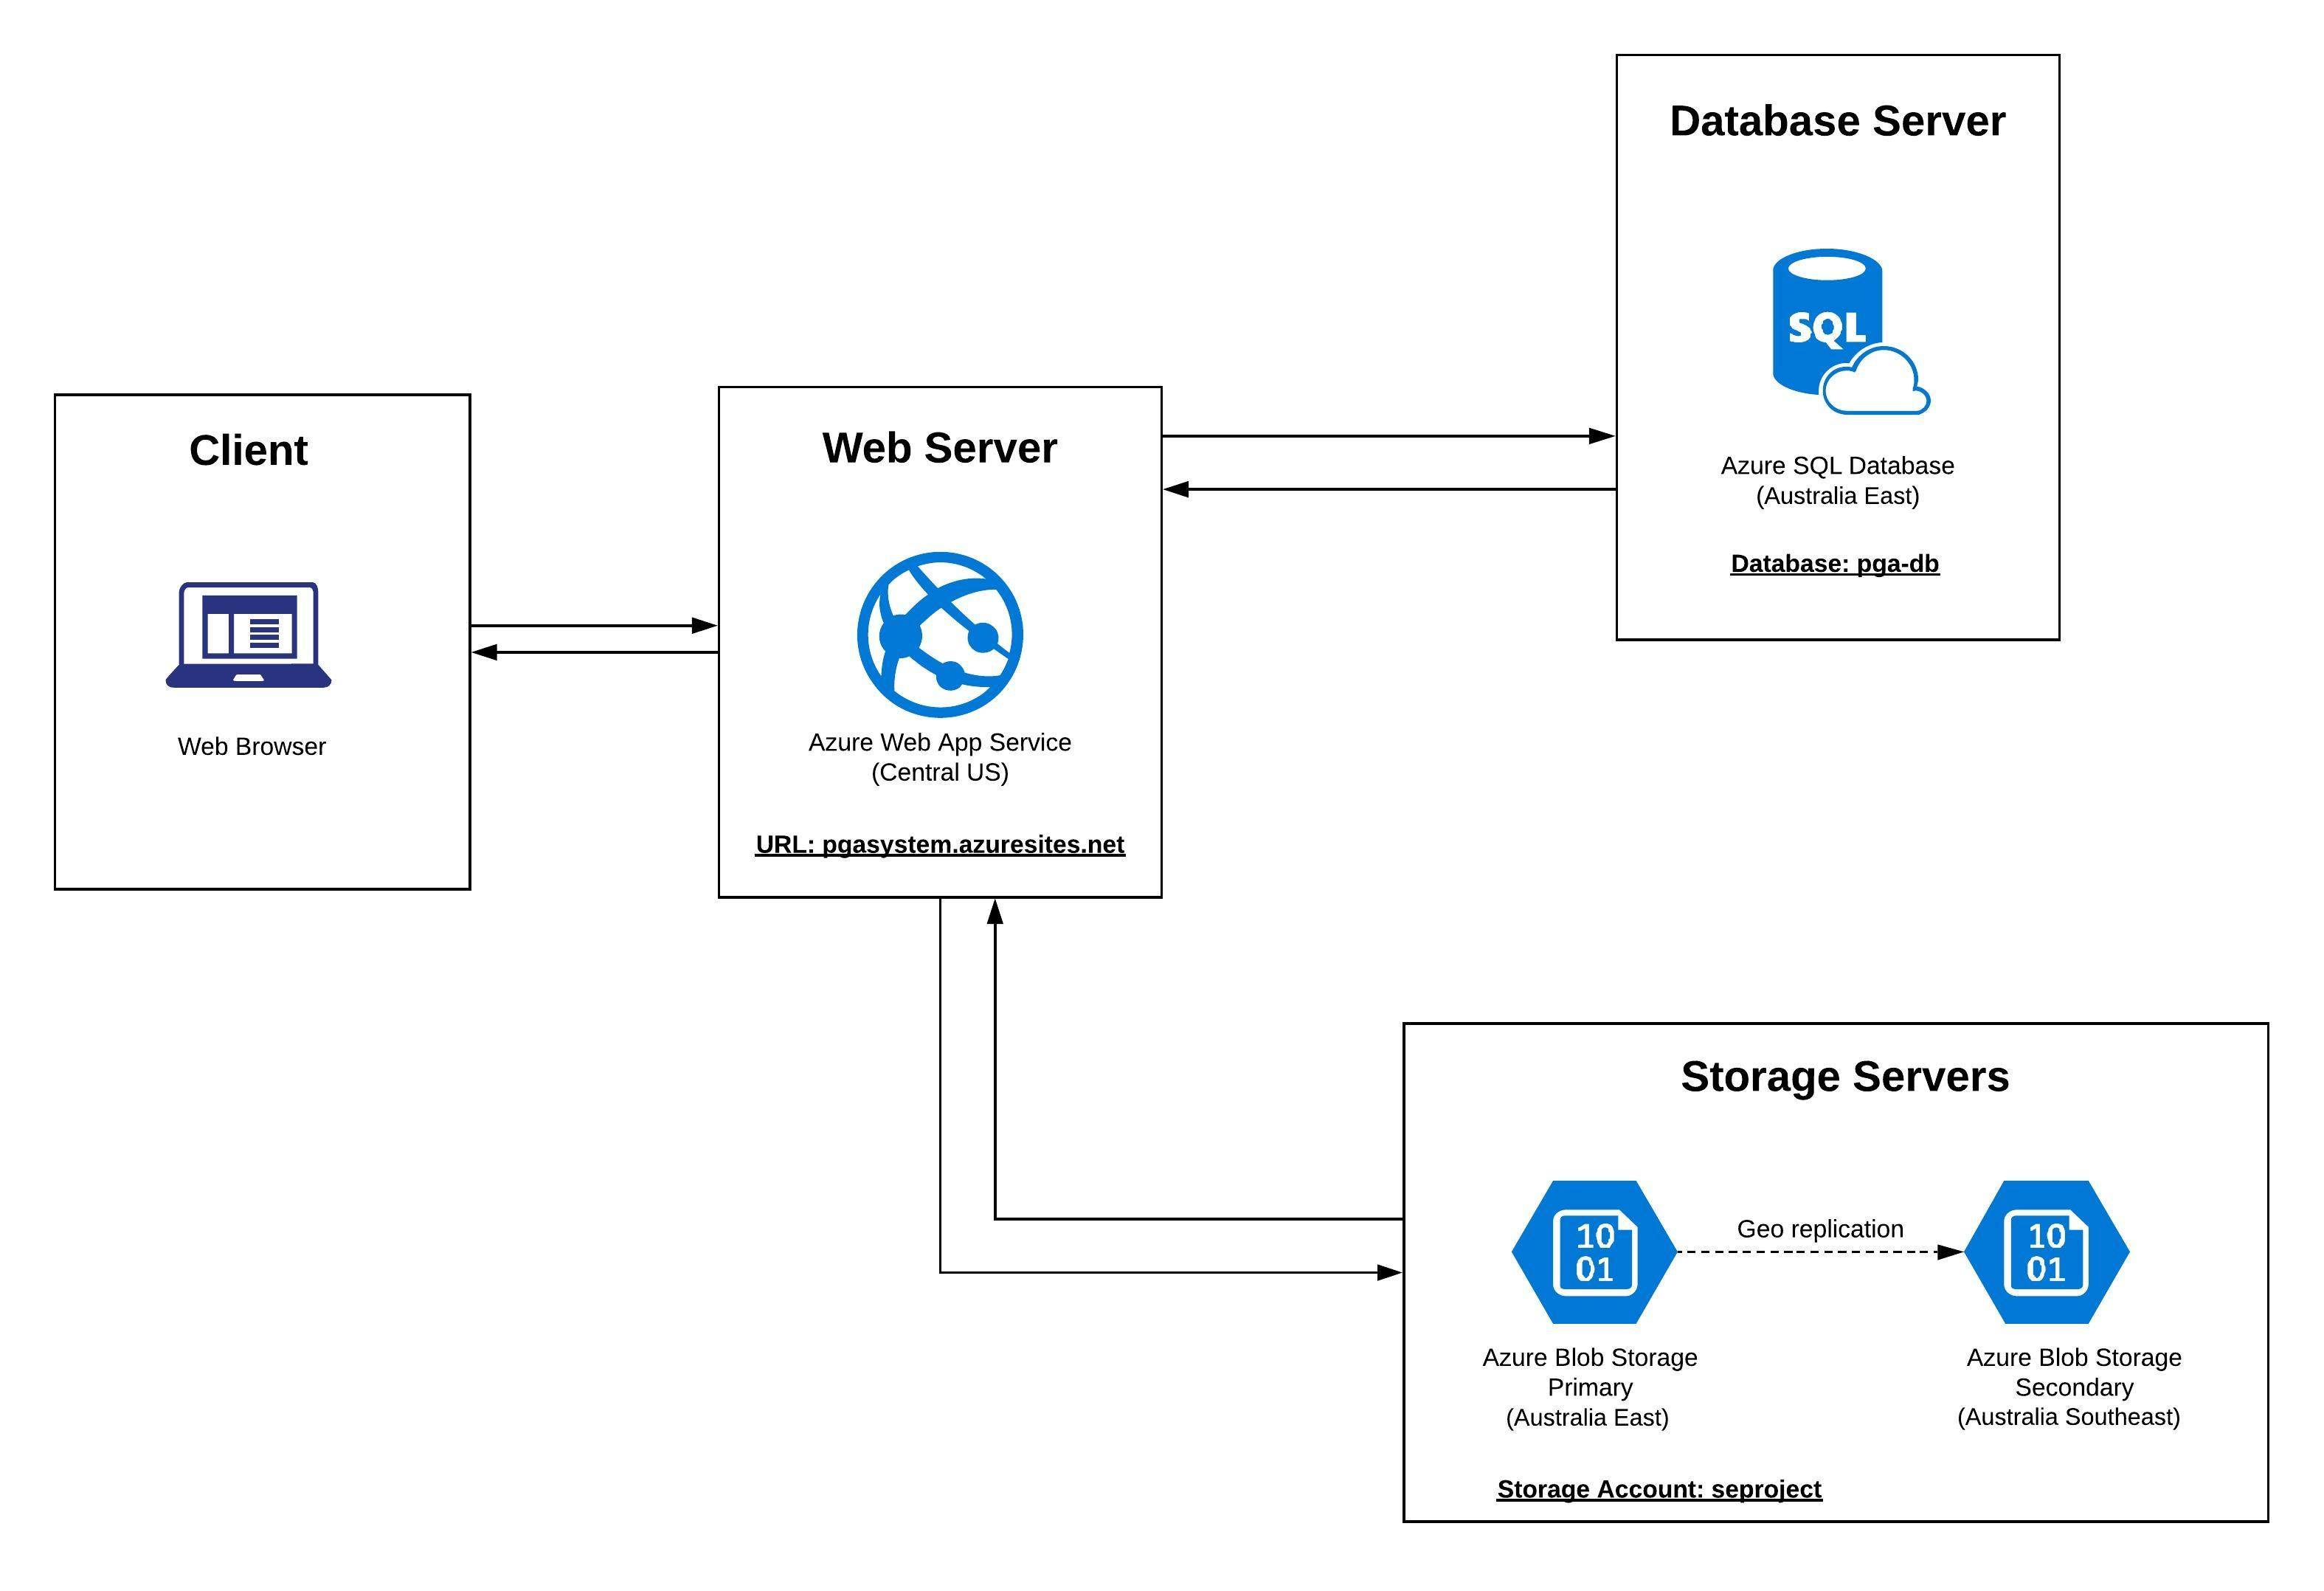
\includegraphics[width=\textwidth, height=\textheight, keepaspectratio]{Diagrams/HardwareArchitecture}}
	\caption{Hardware Architecture Diagram}
\end{figure}
\paragraph{Description}
The hardware architecture consists of:

\begin{itemize}
\item The clients web browser as the layer presenting the PGA System.
\item An Azure web app service that hosts and executes the ASP.NET Core MVC web application (PGA System).
\item An Azure Database server that contains a SQL database where application details are stored. 
\item An Azure Blob Storage server where application documents are stored.

\end{itemize}
\subsection{Process View}
The following activity diagrams describe the dynamic interactions of the two most architecturally significant use cases, namely, Create Application and Update Application.
\subsubsection{Create Application}

\begin{figure}[H]
	\frame{\includegraphics[width=\textwidth, height=\textheight, keepaspectratio]{"Diagrams/ActivityDiagramCreateApplication"}}
	\caption{Activity Diagram for the Create Application Use Case}
\end{figure}
\subsubsection{Update Application}
\begin{figure}[H]
	\frame{\includegraphics[width=\textwidth, height=\textheight, keepaspectratio]{"Diagrams/ActivityDiagramUpdateApplication"}}
	\caption{Activity Diagram for the Update Application Use Case}
\end{figure}
\subsection{Component View}
This section describes the User Interface for each user:

\subsubsection{Common User Screens}
\begin{figure}[H]
	\frame{\includegraphics[width=\textwidth, height=\textheight, keepaspectratio]{"Diagrams/Loginscreen"}}
	\caption{The Login Page}
\end{figure}
\subsubsection{Post Graduate Officer}
\begin{figure}[H]
	\frame{\includegraphics[width=\textwidth, height=\textheight, keepaspectratio]{"Diagrams/PGOHomePage"}}
	\caption{
		The PGO Logs in and lands on this screen.}
\end{figure}
\begin{figure}[H]
	\frame{\includegraphics[width=\textwidth, height=\textheight, keepaspectratio]{"Diagrams/CreateApplication"}}
	\caption{
		The PGO lands here when they click Create Application.}
\end{figure}


\begin{figure}[H]
	\frame{\includegraphics[width=\textwidth, height=\textheight, keepaspectratio]{"Diagrams/PGOViewApplications"}}
	\caption{The PGO lands here when they click Pending Applications from the home page. Here a list of applications with pending decisions, from either a Supervisor or the PGC, is displayed.}
\end{figure}
\begin{figure}[H]
	\frame{\includegraphics[width=\textwidth, height=\textheight, keepaspectratio]{"Diagrams/PGOViewApplication"}}
	\caption{Once the PGO selects an application to view, this screen is displayed. It displays applicant and application information as well as a file viewer.}
\end{figure}
\begin{figure}[H]
	\frame{\includegraphics[width=\textwidth, height=\textheight, keepaspectratio]{"Diagrams/PGOCompletedApplications"}}
	\caption{This page displays applications where the PGC has made a final decision.}
\end{figure}

\subsubsection{Supervisor}
\begin{figure}[H]
	\frame{\includegraphics[width=\textwidth, height=\textheight, keepaspectratio]{"Diagrams/SupervisorHomePage"}}
	\caption{The Landing Page for a Supervisor}
\end{figure}

\begin{figure}[H]
	\frame{\includegraphics[width=\textwidth, height=\textheight, keepaspectratio]{"Diagrams/SupervisorViewApplications"}}
	\caption{The Supervisor can see all pending applications that need their decision.}
\end{figure}
\begin{figure}[H]
	\frame{\includegraphics[width=\textwidth, height=\textheight, keepaspectratio]{"Diagrams/SupervisorViewApplication"}}
	\caption{The view application page for the Supervisor. It displays applicant and application information, a file viewer and a decision picker.}
\end{figure}
\subsubsection{Post Graduate Coordinator}
\begin{figure}[H]
	\frame{\includegraphics[width=\textwidth, height=\textheight, keepaspectratio]{"Diagrams/PGCHomePage"}}
	\caption{The Landing Page for the PGC}
\end{figure}

\begin{figure}[H]
	\frame{\includegraphics[width=\textwidth, height=\textheight, keepaspectratio]{"Diagrams/PGCViewApplications"}}
	\caption{The PGC can see all pending applications that have been accepted by a Supervisor that need final approval.}
\end{figure}
\begin{figure}[H]
	\frame{\includegraphics[width=\textwidth, height=\textheight, keepaspectratio]{"Diagrams/PGCViewApplication"}}
	\caption{The view application page for the PGC. It displays applicant and application information, a file viewer and a decision picker.}
\end{figure}

\subsection{Database View}
This section contains the Entity-Relationship Diagram for the System Database:
\begin{figure}[H]
	\frame{\includegraphics[width=\textwidth, height=\textheight, keepaspectratio]{"Diagrams/PGASEntityRelationshipDiagram"}}
	
\end{figure}


\section{Performance and Unit Testing}

\subsection{Performance Test Details and Results} 
A stress test was conducted on the system. The Microsoft Azure performance testing framework was used. 
The stress test simulated 40 concurrent users, each sending an average of 5 requests per second for a full minute.
The test results were as follows:
\begin{itemize}
	\item Average response time: 0.08 seconds
	\item Average total requests per second: 194.67
	\item Total requests: 10927
	\item Successful requests: 10927
	\item Failed requests: 0 
\end{itemize}
\subsection{Unit Testing}
A total of four test cases were implemented to show the feasibility of the testing framework. In future development of the system, it is expected that many more Unit tests will be implemented.

The following Unit Test Scenarios have been tested:

\begin{itemize}
\item Get Application:

This scenario ensures that users can view applications seemlessly when required. Two test cases are used to achieve this. The first test checks if the system returns a valid applicant by passing an application Id. The second test, tests that system throws a valid exception with a description if an invalid (negative id or non-existent) applicationId is accessed. Both these tests ensure that the prototype functions correctly in every scenario that requires it to retrieve an application.


\item Get Files:

This scenario ensures that all corresponding applicant documents can be viewed by the user. Three test cases are used to achieve this. The first test tests if the correct number of files is returned for valid application Id. This is important to ensure that files from an applicant do not go missing. The second case tests if the correct file data is returned for valid application Id. This is important to ensure that documents from applicants do not get mixed up. Lastly, the third test tests if a valid exception is thrown if an application does not exist. All these tests in conjunction ensure that the prototype works correctly when required to retrieve application files.


\item Add Application:

This scenario tests whether a PGO can add an application to the system without any errors. One test case is used for this, which tests if the application has been added to the context. This is important as the test will fail if the application is not added and hence it ensures that applications do not go missing when added to the system.


\item Get Supervisor:

This scenario tests if a valid supervisor is returned when requested by passing a supervisor Id. This ensures that supervisors can be correctly allocated and notified when required. Two test cases are used to achieve this. The first tests if a valid supervisor is returned when entering a supervisor id and the second tests if an error is thrown if an invalid supervisor Id is entered. This is important to ensure that supervisors are correctly identified by their Id in the system.


\end{itemize}



\end{document}

